
\begin{frame}
\newcommand{\song}{\setCJKfamilyfont{song}}
\newcommand{\xiaoer}{\fontsize{18pt}{18pt}\selectfont}
	\begin{center}
	{\song\xiaoer\textbf{人工鱼群算法}}
	\end{center}
\end{frame}

\begin{frame}
	\frametitle{目录}
	\begin{itemize}
		\item{算法背景}
		\item{算法简介}
		\item{算法实现}
		\item{算法应用}
		\item{分析思考}
		\item{参考文献}

	\end{itemize}
\end{frame}

\begin{frame}
	\frametitle{算法背景}
	\begin{itemize}
		\item{提出者:李晓磊等,2002年}
		\item{提出背景:随着人工智能和人工生命的兴起,出现了一些仿生算法,包括蚁群算法和粒子群算法等。将人工智能的思想应用于问题的寻优,实施一些高级的计算方法。应用动物自治体的模式来定义实体,让他们在问题空间中自主的活动,从而达到解决问题的目的。}
	\end{itemize}
\end{frame}

\begin{frame}
	\frametitle{算法简介}
	\begin{itemize}
		\item{鱼群模式}
			\begin{itemize}
				\item{视觉}
				\item{鱼群行为分析}
				\item{人工鱼}
				\item{问题解决}
			\end{itemize}
		\item{人工鱼模型}
		\item{行为描述}
	\end{itemize}
\end{frame}

\begin{frame}
	\frametitle{鱼群模式——视觉}
	\begin{columns}
	\column{.5\textwidth}
		\begin{figure}
			\centering
			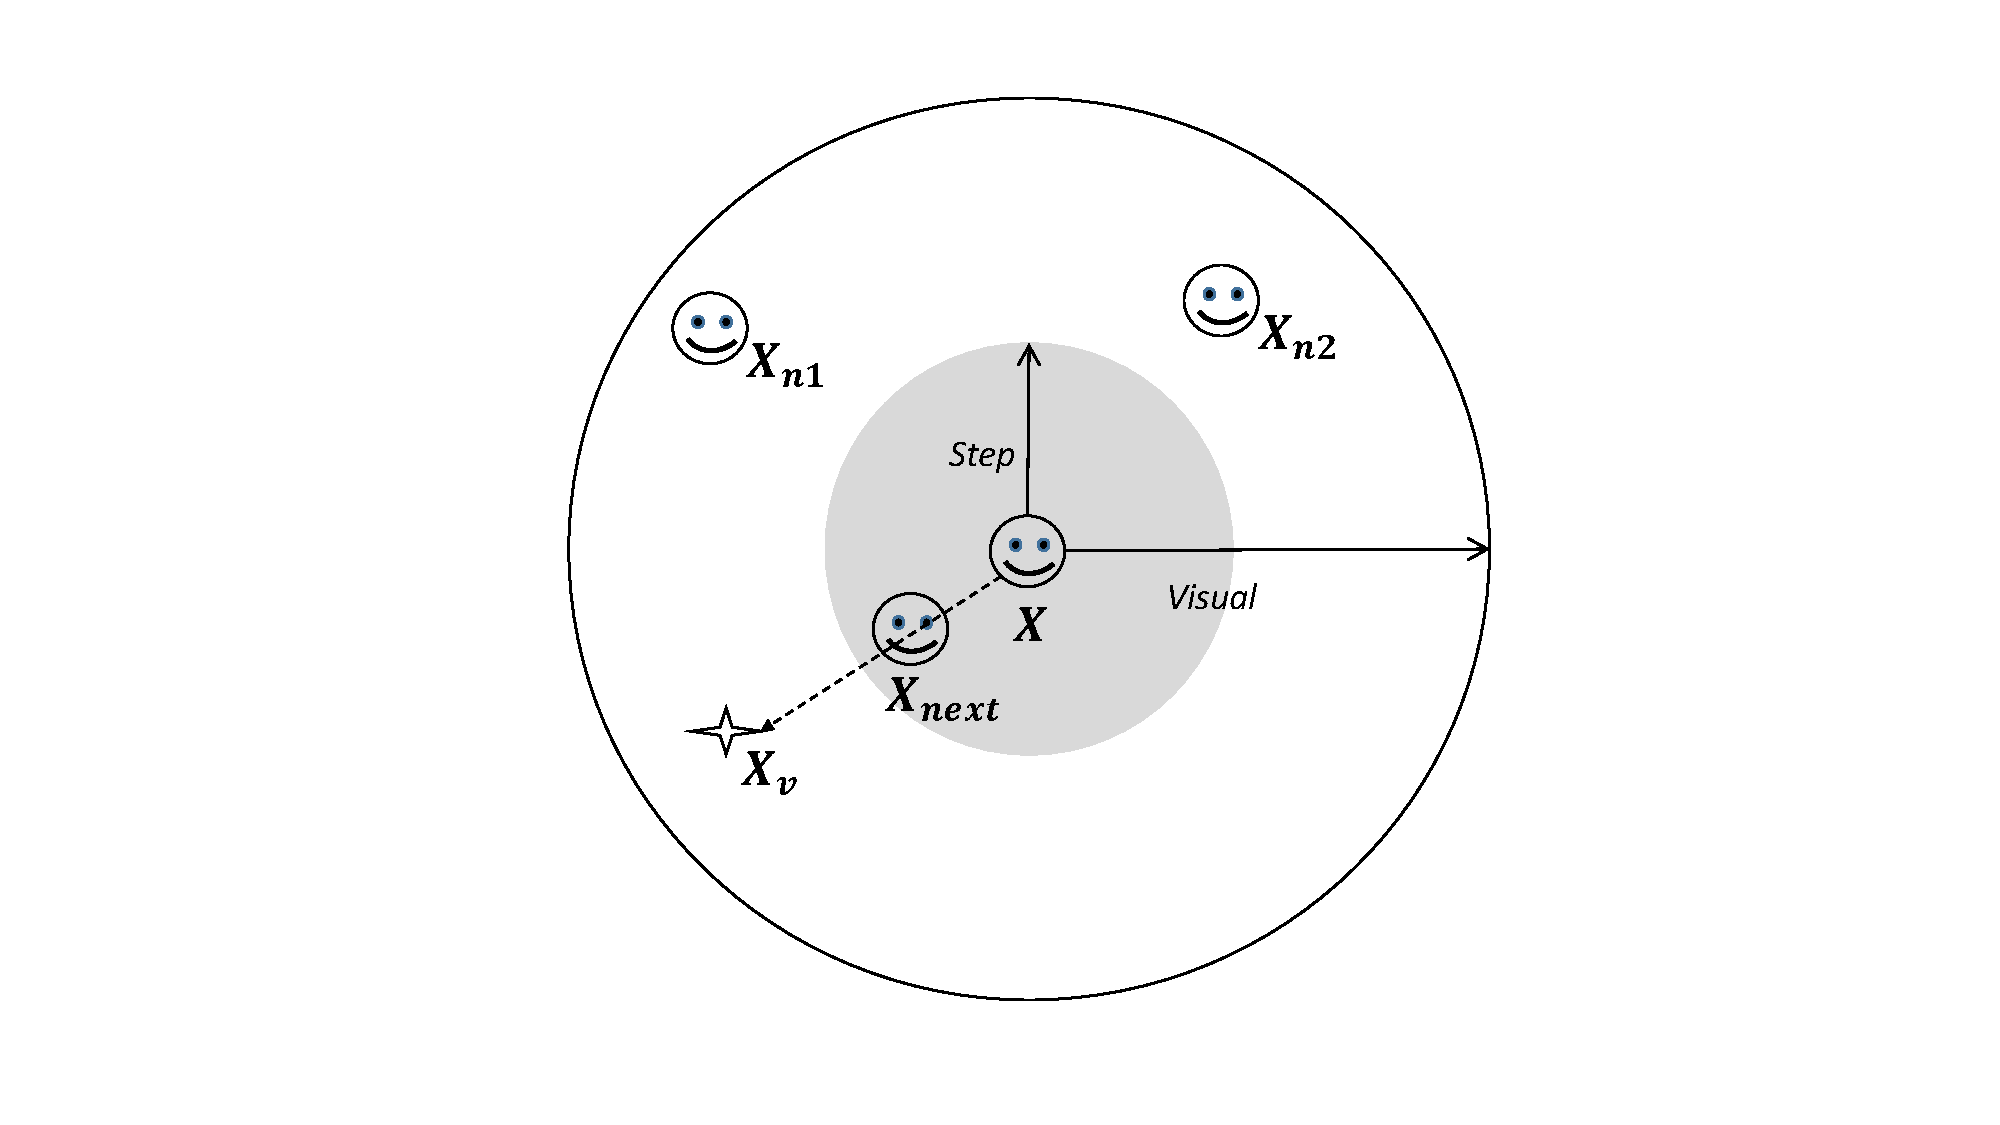
\includegraphics[width=0.9\textwidth]{pic/fish1.pdf}
			\caption{人工鱼的视野和移动步长}
		\end{figure}
	\column{.5\textwidth}
	虚拟人工鱼实体的当前状态为X,Visual为其视野范围,状态$X_v$为其在某时刻视点所在的位置,如果该位置的状态优于当前状态,则考虑向该位置方向前进一步,即到达状态$X_{next}$
	\end{columns}
\end{frame}

\begin{frame}
	\frametitle{鱼群模式——鱼群行为分析}
	\begin{columns}
	\column{.5\textwidth}
		\begin{itemize}
			\item{聚群行为:鱼类进化过程中的一种生存方式,大量或少量的鱼都能聚集成群,进行集体觅食和躲避敌害}
			\item{追尾行为:当某一条鱼或几条鱼发现食物时,它们附近的鱼会尾随其后快速游过来,进而导致更远处的鱼也尾随过来}
		\end{itemize}
	\column{.5\textwidth}
		\begin{itemize}
			\item{随机行为:鱼在水中悠闲的自由游动,基本上是随机的,其视也是为了更大范围地寻觅食物或同伴}
			\item{觅食行为:生物的基本行为,趋向食物的一种活动。一般可以认定它是同过视觉或味觉来感知水中的食物量或浓度来选择趋向}
		\end{itemize}
	\end{columns}
\end{frame}

\begin{frame}
	\frametitle{鱼群模式——人工鱼}
	\begin{columns}
	\column{.6\textwidth}
		\begin{figure}
			\centering
			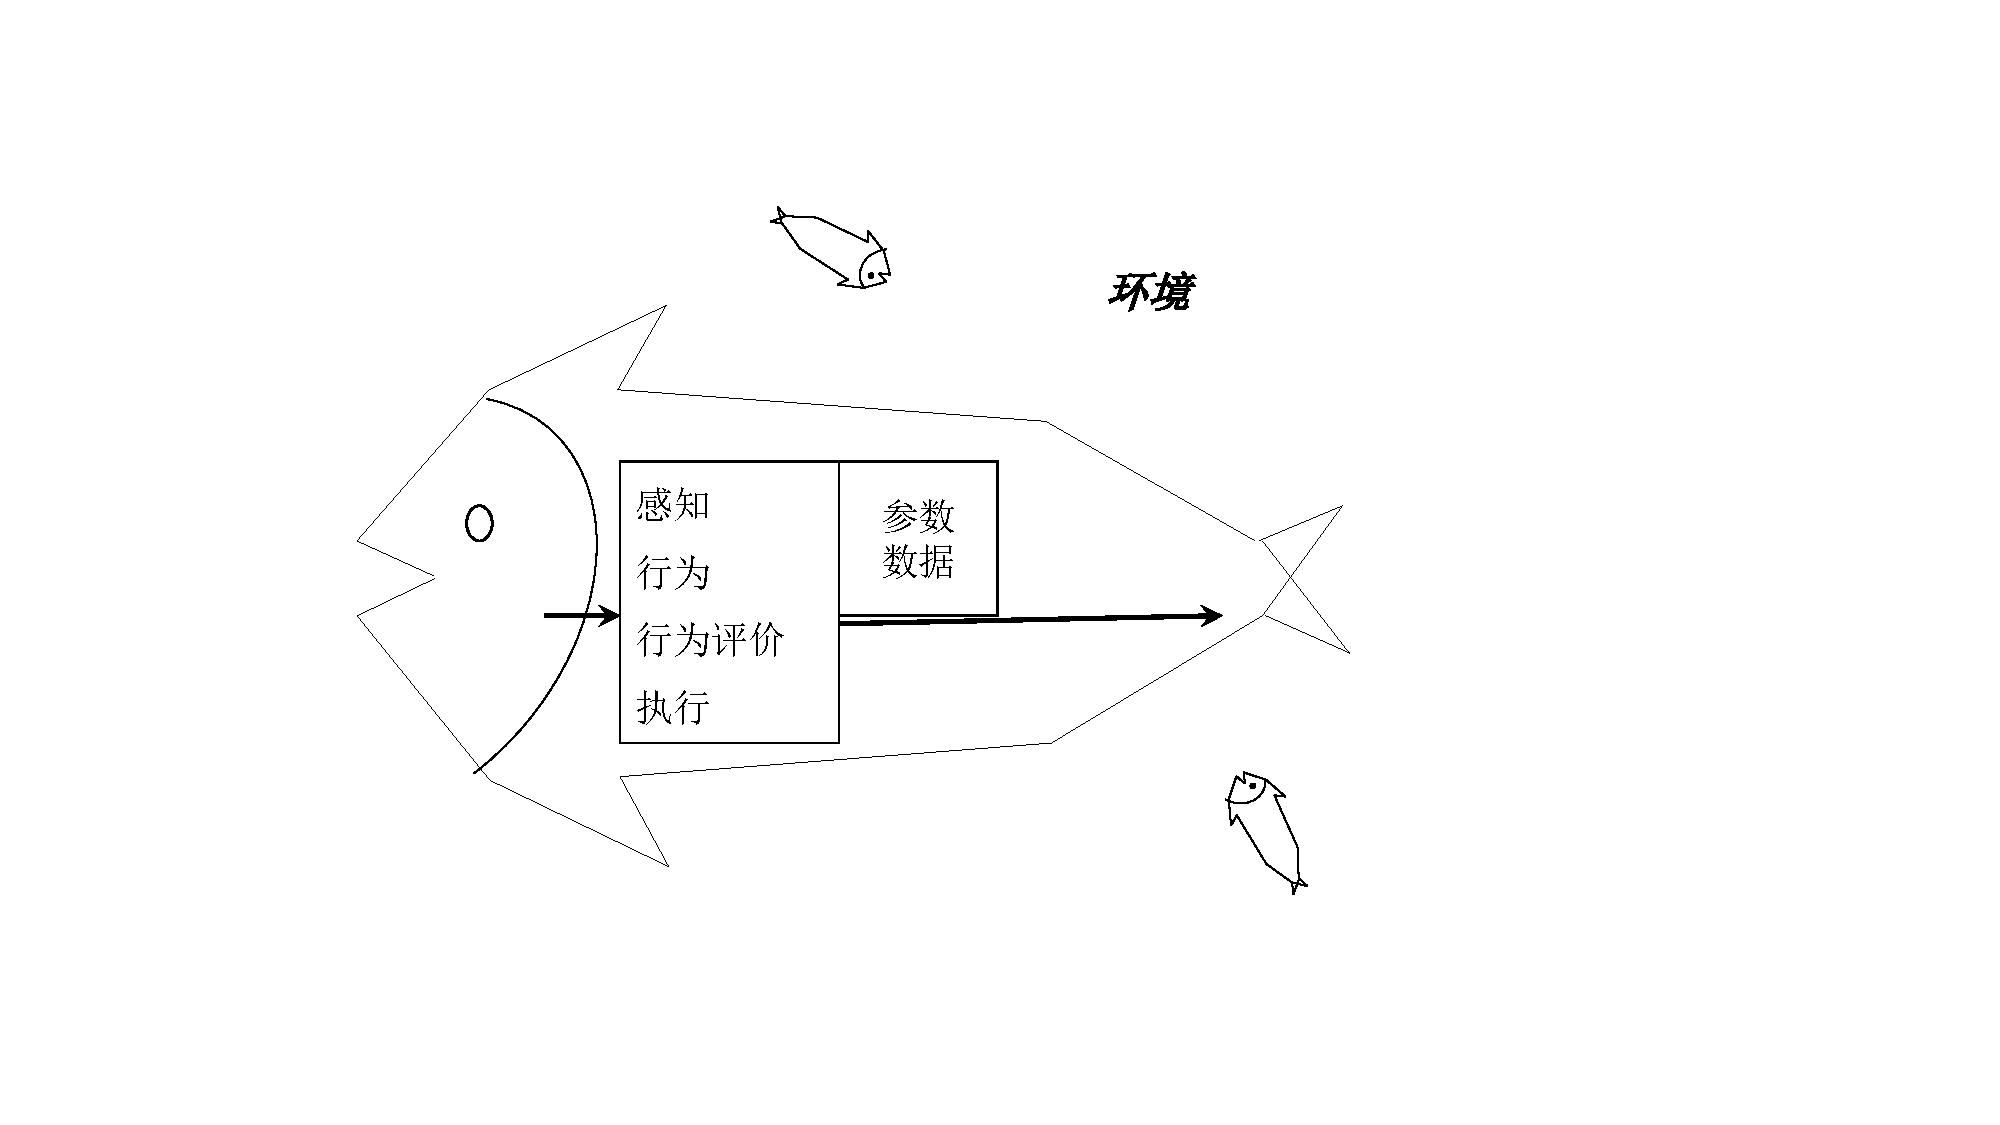
\includegraphics[width=0.9\textwidth]{pic/fish2.pdf}
			\caption{人工鱼实体}
		\end{figure}
	\column{.4\textwidth}
		人工鱼是真实鱼个体的一个虚拟实体,用来进行问题的分析和说明。\\如图所示,可以将人工鱼看作是一个封装了自身数据星系和一系列行为的一个实体,同过感官来接受环境的刺激信息,并通过控制尾鳍来做出相应的应激活动。\\人工鱼所在的环境主要是问题的解空间和其他人工鱼的状态,它在下一刻的行为取决于目前自身状态和目前环境的状态,并且它还通过自身活动的同时来影响环境,进而影响其他同伴的活动。
	\end{columns}
		
\end{frame}
\begin{frame}
	\frametitle{鱼群模式——问题解决}
	实际问题的解决是通过自治体在自主的活动过程中以某种形式表现出来的。在一片水域中,鱼生存的数目最多的地方一般就是本水域中富含营养物质最多的地方,依据这一特点来模仿鱼群的觅食等行为,从而实现全局寻优,这就是鱼群算法的基本思想。\\在寻优过程中,通常会有两种方式表现出来:
	\begin{itemize}
		\item{一种形式是通过人工鱼最终的分布情况来确定最优解的分布,通常随着寻优解过程的进展,人工鱼往往会聚集在极值点的周围,而且,全局最优的极值点周围能聚集较多的人工鱼}
		\item{另一种形式是在人工鱼的个体状态之中表现出来的,即在寻优的过程中,跟踪记录最优个体的状态,类似于遗传算法等的方式}
	\end{itemize}
\end{frame}
\begin{frame}
	\frametitle{人工鱼模型}
	\begin{columns}
	\column{.35\textwidth}
	\flushleft
		\small{\emph{{class Artificial\underline{\hspace{0.5em}}fish}\\{\{}\\Various:\\{\qquad{float AF\underline{\hspace{0.5em}}X[n];}}\\{\qquad{float AF\underline{\hspace{0.5em}}step;}}\\{\qquad{float AF\underline{\hspace{0.5em}}visual;}}\\{\qquad{float try\underline{\hspace{0.5em}}number}}\\{\qquad{float delta;}}\\{Functions:}\\{\qquad{float AF\underline{\hspace{0.5em}}foodconsistence();}}\\{\qquad{void AF\underline{\hspace{0.5em}}move();}}\\{\qquad{float AF\underline{\hspace{0.5em}}follow();}}\\{\qquad{float AF\underline{\hspace{0.5em}}prey();}}\\{\qquad{float AF\underline{\hspace{0.5em}}swarm();}}\\{\qquad{int AF\underline{\hspace{0.5em}}evaluate();}}\\{\qquad{void AF\underline{\hspace{0.5em}}init();}}\\{\qquad{Artificial\underline{\hspace{0.5em}}fish();}}\\{\qquad{virtual~Artificial\underline{\hspace{0.5em}}fish;}}\\{\};}}}
	\column{.45\textwidth}
	\flushleft
		\small{\emph{ \vspace{0.5ex}\\{//AFs positon}\\//the distance that AF can move for each step\\//the visual distance of AF\\//attempt time in the behavior of prey\\//the condition of jamming\vspace{3ex}\\//the food consistence of AFs current position\\//AF move to the next position\\//the behavior of follow\\//the behavior of prey\\//the behavior of swarm\\//evaluate and select the behavior\\//to initialize the AF\vspace{3ex} }}
	\column{.2\textwidth}
		\tiny{Step:人工鱼移动最大步长\\{$\delta:$拥挤度因子}\\Visual:人工鱼感知距离\\个体状态:$(x_1,x_2,···,x_n)$,其中$x_i$为欲寻优的变量\\Y=f(X)表示当前所在位置食物浓度\\人工鱼个体之间的距离:$d_{i,j}=|X_i-X_j|$}
	\end{columns}
\end{frame}
\begin{frame}
	\frametitle{行为描述}
		\begin{columns}
		
		\column{0.55\textwidth}
		\small{觅食行为}\vspace{3ex}\\
			\flushleft\scriptsize{\emph{float Aritificial\underline{\hspace{0.5em}}fish::AF\underline{\hspace{0.5em}}prey()\\{\{}\\{\qquad for($i=0;i<try\underline{\hspace{0.5em}}number;i++)$}\\{\qquad\{}\\{\qquad\qquad$X_j=X_i+Rand()·Visual;$}\\{\qquad\qquad if $(Y_i<Y_j)$}\\{\qquad\qquad\qquad $X_{i|next}=X_i+Rand()·Step·(X_j-X_i)/\lVert X_j-X_i\rVert;$}\\{\qquad\qquad else}\\{\qquad\qquad\qquad $X_{i|next}=X_i+Rand()·Step;$}\\{\qquad\}}\\{ return $AF\underline{\hspace{0.5em}}foodconsistence(X_{i|next});$} \\{\}} }}
		\column{0.55\textwidth}
		\small{聚群行为}\vspace{3ex}\\
			\flushleft\scriptsize{\emph{float Aritificial\underline{\hspace{0.5em}}fish::AF\underline{\hspace{0.5em}}swarm() \\ {\{} \\ {\qquad $n_f=0;X_c=0$} \\ {\qquad for($j=0;i<friend\underline{\hspace{0.5em}}number;j++)$} \\ {\qquad\qquad $if(d_{i.j}<Visual) \{ n_f++;X_c+=X_j;\}$} \\ {\qquad $X_c=X_c/n_f;$}\\{\qquad $if (Y_c/n_f>\delta Y_i)$}\\{\qquad\qquad $X_{i|next}=X_i+Rand()·Step·(X_c-X_i)/\lVert X_c-X_i\rVert;$}\\{\qquad else}\\{\qquad\qquad AF\underline{\hspace{0.5em}}prey();}\\{ return $AF\underline{\hspace{0.5em}}foodconsistence(X_{i|next});$} \\{\}} }}
		\end{columns}
		
\end{frame}

\begin{frame}
	\frametitle{行为描述}
		\begin{columns}
		\column{0.6\textwidth}
		\small{追尾行为}\vspace{3ex}\\
			\flushleft\scriptsize{\emph{float Aritificial\underline{\hspace{0.5em}}fish::AF\underline{\hspace{0.5em}}follow() \\ {\{} \\ {\qquad $Y_max=-\infty;$} \\ {\qquad for($j=0;i<friend\underline{\hspace{0.5em}}number;j++)$} \\ {\qquad\qquad $if(d_{i,j}<Visual \&\& Y_j>Y_max)$} \\ {\qquad\qquad\qquad $\{ Y_max=Y_j; X_max=X_j; \}$ }\\{\qquad $n_f=0$}\\{\qquad for($j=0;i<friend\underline{\hspace{0.5em}}number;j++)$}\\{\qquad\qquad $if(d_{max,j}<Visual) \{ n_f++;\} $}\\{\qquad $if (Y_max/n_f>\delta Y_i)$}\\{\qquad\qquad $X_{i|next}=X_i+Rand()·Step·(X_max-X_i)/\lVert X_max-X_i\rVert;$}\\{\qquad else}\\{\qquad\qquad AF\underline{\hspace{0.5em}}prey();}\\{ return $AF\underline{\hspace{0.5em}}foodconsistence(X_{i|next});$} \\{\}} }}
		\column{0.4\textwidth}
		\small{随机行为}\vspace{3ex}\\
		\vspace{6ex}随机行为的实现即在视野中随机选择一个状态,然后向该方向移动,实际上就是觅食行为的一个缺省行为。
		\end{columns}
\end{frame}

\begin {frame}
	\frametitle{算法描述}
		\begin{columns}
		\column{0.5\textwidth}
		\begin{figure}
			\centering
			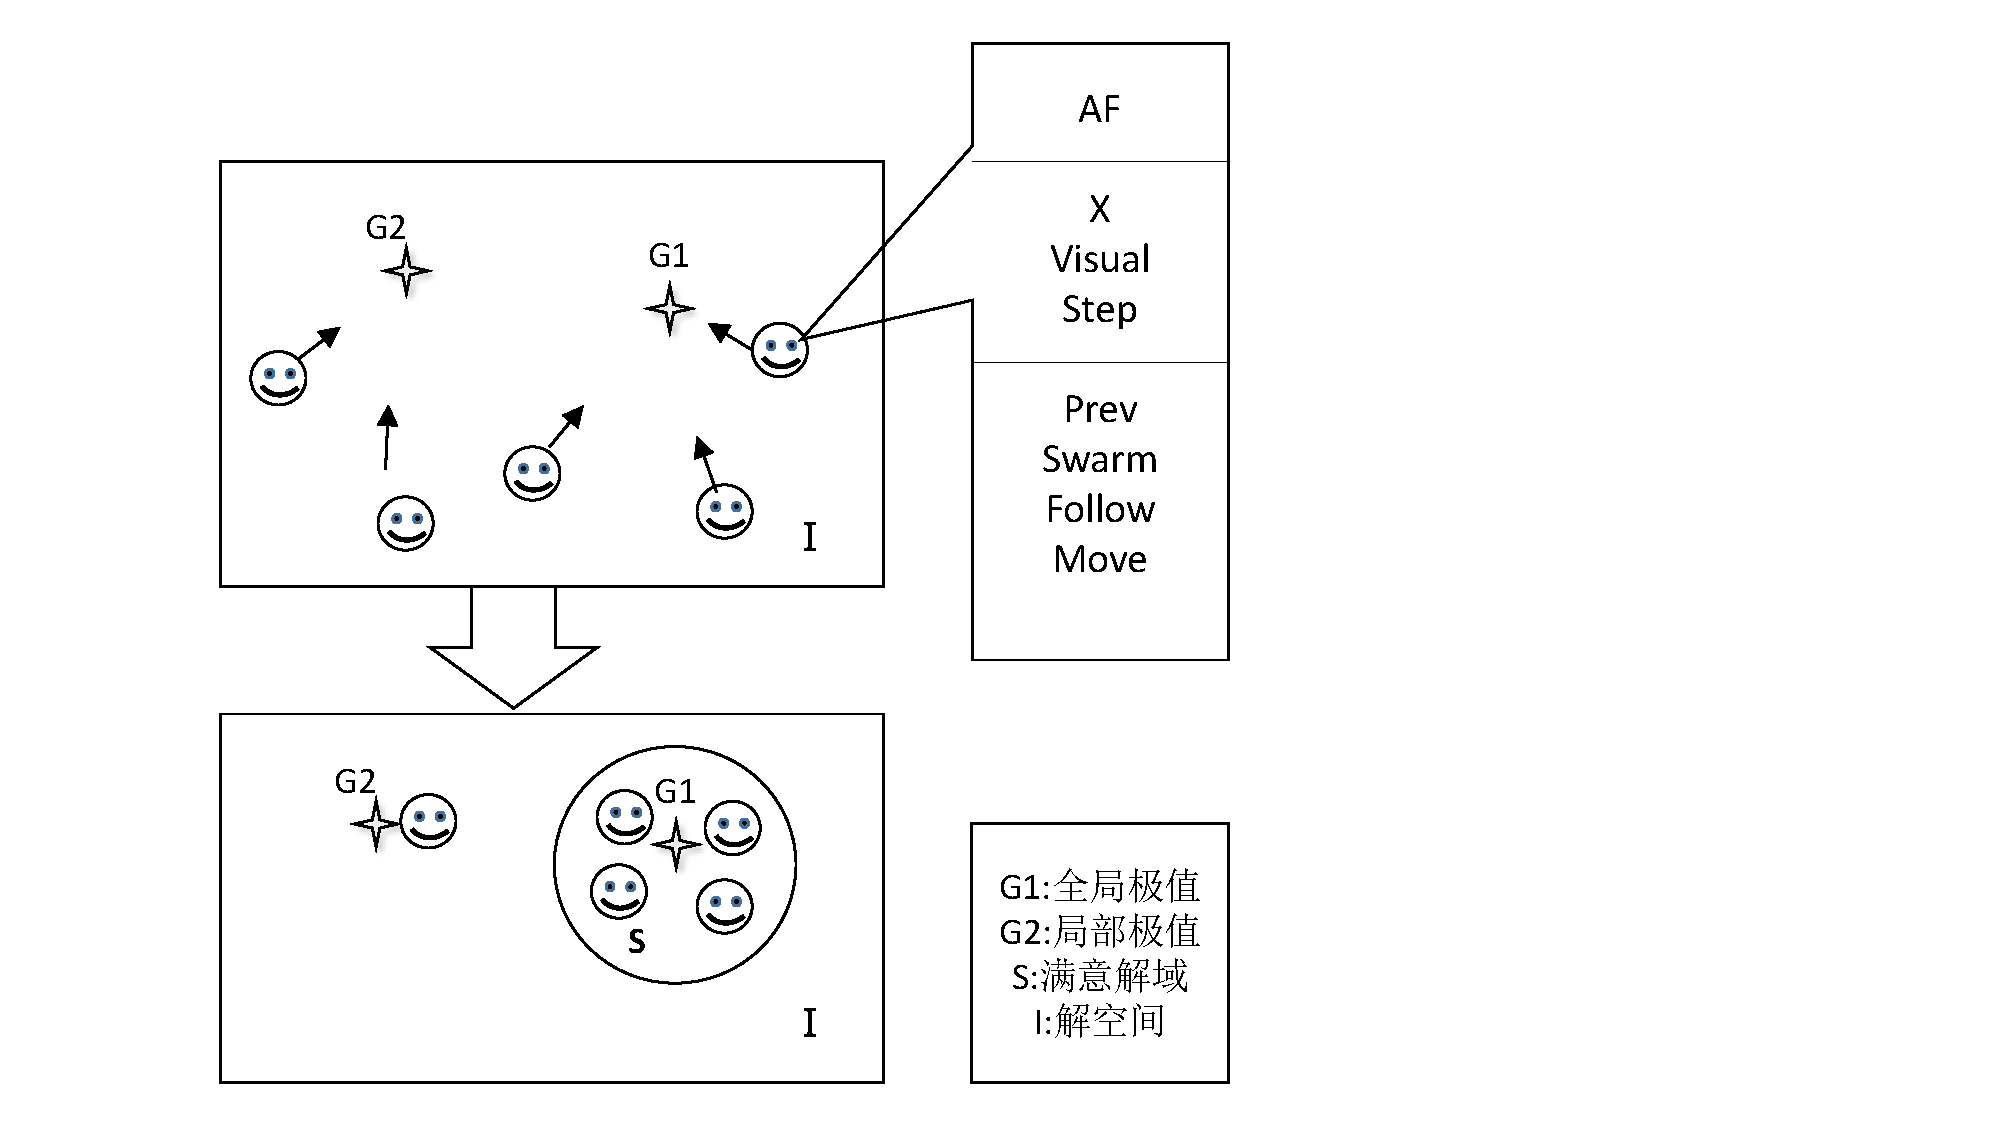
\includegraphics[width=0.8\textwidth]{pic/fish3.pdf}
			\caption{算法示意图}
		\end{figure}
		
		\column{0.5\textwidth}
		\small{每个人工鱼探索它的环境状况(包括目标函数的变化情况和伙伴的变化情况),从而选择一种行为\\最终,人工鱼集结在几个局部极值的周围\\一般情况下,在讨论求极大问题时,拥有较大的$AF\underline{\hspace{0.5em}}foodconsistence$值的人工鱼一般处于值较大的极值域周围\\这有助于获取全局极值域,而值较大的极值区域周围一般能集结较多的人工鱼,这有助于判断并获取全局极值。}
		\end{columns}

\end{frame}

\begin{frame}
	\frametitle{算法实现}
	\begin{algorithm}[H]
	\caption{AFA算法}\label{fish_alg}
	\algsetup{linenosize=\tiny} \scriptsize
		\begin{algorithmic}
			\STATE{$AF\underline{\hspace{0.5em}}init()$}
			\WHILE{the resulr is satisfied}
				\STATE{\textbf{switch}$(AF\underline{\hspace{0.5em}}evaluat())$}	
				\STATE{\textbf{\quad case}\quad value1:}
				\STATE{$\qquad AF\underline{\hspace{0.5em}}follow()$}
				\STATE{\textbf{\quad case}\quad value1:}
				\STATE{\qquad $AF\underline{\hspace{0.5em}}swarm()$}
				\STATE{\quad \textbf{default$:$}}
				\STATE{\qquad $AF\underline{\hspace{0.5em}}prey()$}
				\STATE{\textbf{end switch}}			
				\STATE{$AF\underline{\hspace{0.5em}}move()$}
				\STATE{$get\underline{\hspace{0.5em}}result()$}
			\ENDWHILE
			
		\end{algorithmic}
	\end{algorithm}
\end{frame}

\begin{frame}
	\frametitle{仿真实验研究}
寻优对象选取了下面的非线性目标函数:\\
	\indent\indent $max f(x,y)=\tfrac {sin(x)}{x}\ \frac{sin{y}}{y}$\\
	\indent\indent $s.t. x\in [-10,10]$\\
	\indent\indent $y\in [-10,10]$\\
	\begin{figure}
		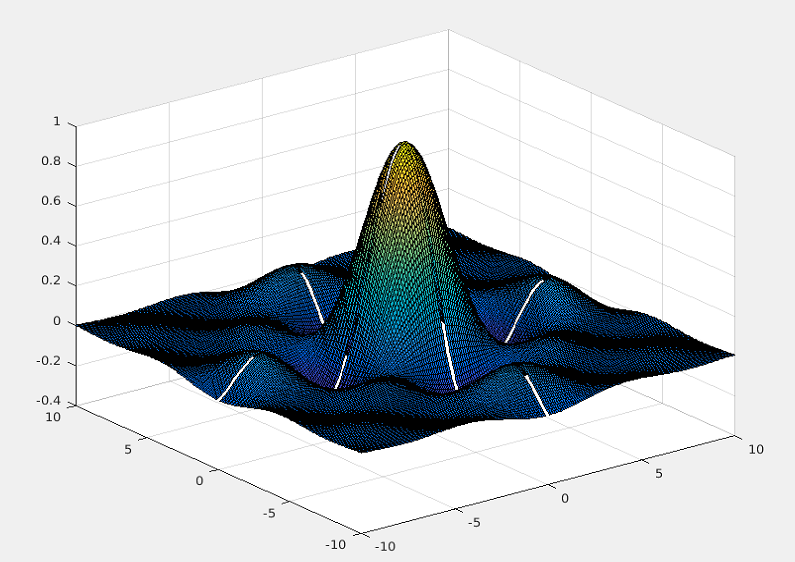
\includegraphics[width=0.4\textwidth]{pic/fish9.png}
		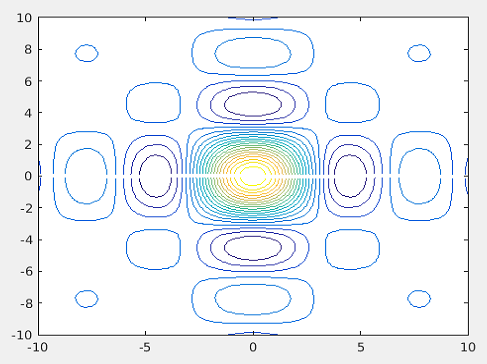
\includegraphics[width=0.4\textwidth]{pic/fish10.png}
		\caption{具有多个局部极值的非线性目标函数}
	\end{figure}
如图所示,可以看出,该非线性函数在全局极大值的周围密布着许多局部极值,通常的寻优算法极易陷入局部极值或在局部极值间震荡,比较适用于验证算法的性能。
\end{frame}

\begin{frame}
\frametitle{仿真结果}
	下面的仿真实验中,AF的数量为10个,为了检验其寻优的效率,令它们的初始位置都处于距全局极值最远的(-10,10)处,其感知距离Visual=2.5,每次移动的步长Step=0.3,拥挤度因子$\delta = 0.618$.
图5为AF只执行聚群行为的仿真结果,(a)中,AF迅速聚集在最近的局部极值点附近,(b)中已经有了AF到达全局极值的附近,(c)中有更多的AF到达了全局极值点的附近,且有少数AF聚集到了其他的局部极值点附近,从寻优曲线可以看出,AF能较快地跳出局部极值点,从而较快地找到全局极值
\begin{figure}[htbp]
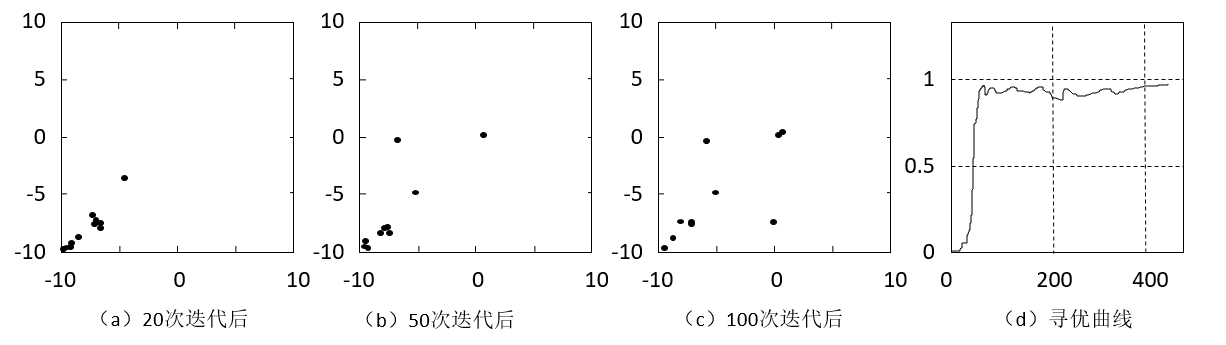
\includegraphics[width=1.0\textwidth]{pic/fish11.png}
\caption{聚群行为的仿真结果}
\end{figure}
\end{frame}
\begin{frame}
\frametitle{仿真结果}
下图为AF只执行追尾行为的仿真结果。如图(a)中,AF迅速聚集在最近的局部极值点附近,图(b)中,AF又迅速向附近的极值点聚集,图(c)中有更多的AF聚集到了附近的局部极值点的附近,并有AF开始到达了全局极值点附近,从寻优曲线可以看出,AF能较快地聚集到某个极值点,但可能会陷于其中。
\begin{figure}[H]
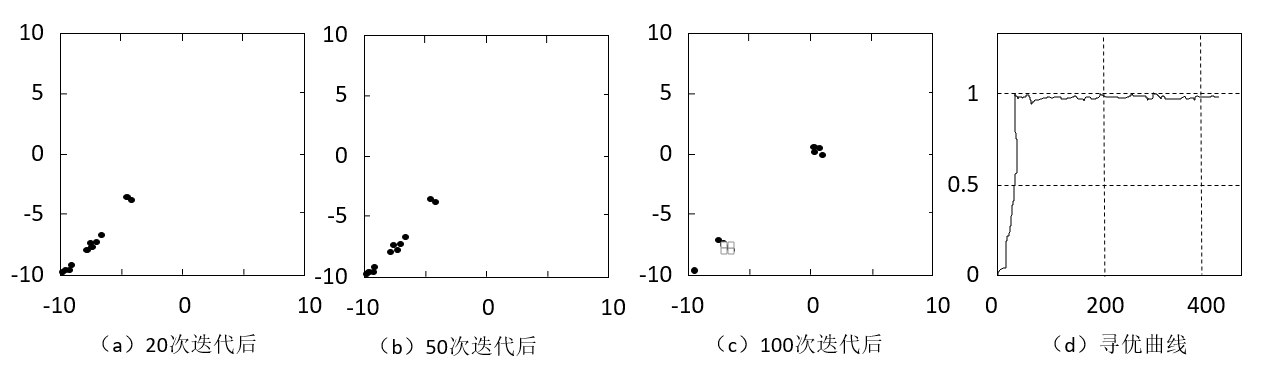
\includegraphics[width=1.0\textwidth]{pic/fish12.png}
\caption{追尾行为的仿真结果}
\end{figure}
\end{frame}
\begin{frame}
\frametitle{仿真结果}
下图为完整的人工鱼群算法的仿真结果,从图中可以看出, AF能迅速向全局极值点附近聚集,从寻优曲线可以看出, AF能很快地搜索到全局极值点并较快地稳定在满意解域内。
\begin{figure}[H]
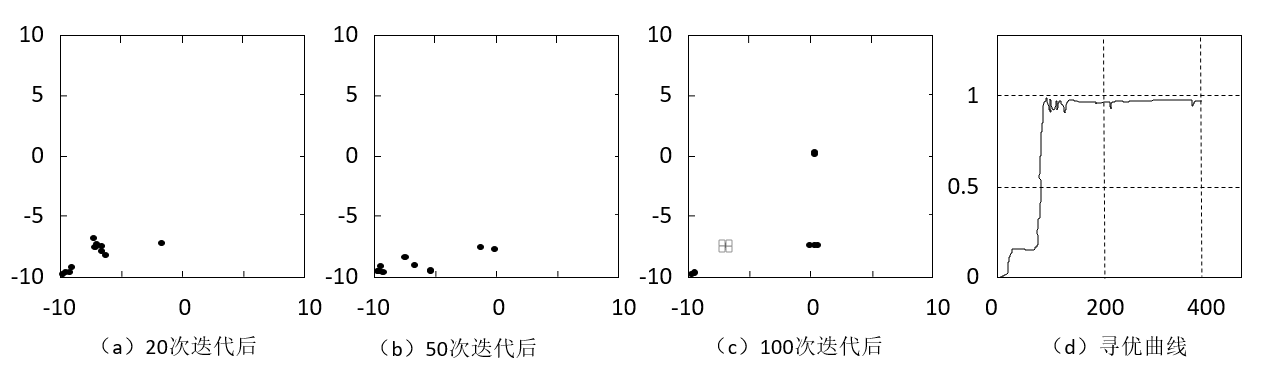
\includegraphics[width=1.0\textwidth]{pic/fish13.png}
\caption{鱼群算法仿真结果}
\end{figure}
\end{frame}

\begin{frame}
\frametitle{仿真结果}
由上可得出如下结论:
\begin{itemize}
\item{聚群行为能够很好地跳出局部极值,并尽可能地搜索到其他的极值,最终搜索到全局极值。}
\item{追尾行为有助于快速的向某个极值方向前进,加快寻优的速度,并防止AF在局部振荡而停滞不前。}
\item{鱼群算法在对以上两种行为进行评价后,自动选择合适的行为,从而形成了一种高效快速的寻优策略。}
\end{itemize}
\end{frame}

\begin{frame}
\frametitle{各参数对计算时间的影响结果}
\small{各参数对计算时间的影响如图所示,可以看出,参数Step、Visual、$\delta$的影响都是有限的,而人工鱼数目的影响通过回归分析可以看出是呈二次函数上升的;对人工鱼的数目与收敛迭代次数关系的回归分析可以看出,AFnumher的增加对迭代次数的减少是呈幂指数下降的,这或许能补偿一下由于人工鱼数目增加而造成的计算量增加的问题,因此,合理选择人工鱼的数目是提高算法效率的关键。这一规律是否具有一般性还有待进一步研究,如与目
标函数的性质有无关系、与算法实现的代码优化有无关系等。}
\begin{figure}
\centering
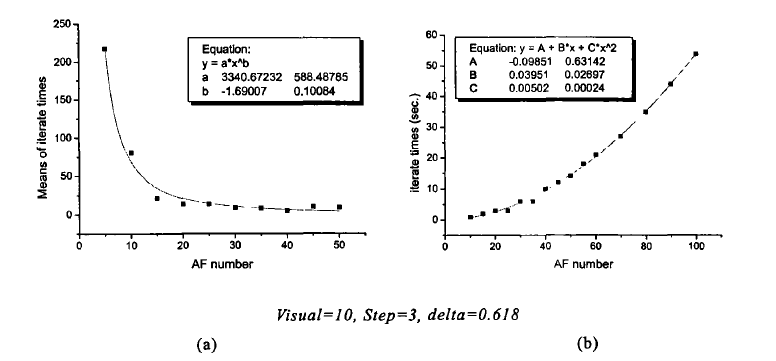
\includegraphics[width=0.6\textwidth]{pic/fish6.png}
\end{figure}
\end{frame}

\begin{frame}
\frametitle{各参数对计算时间的影响结果}
\begin{figure}
\centering
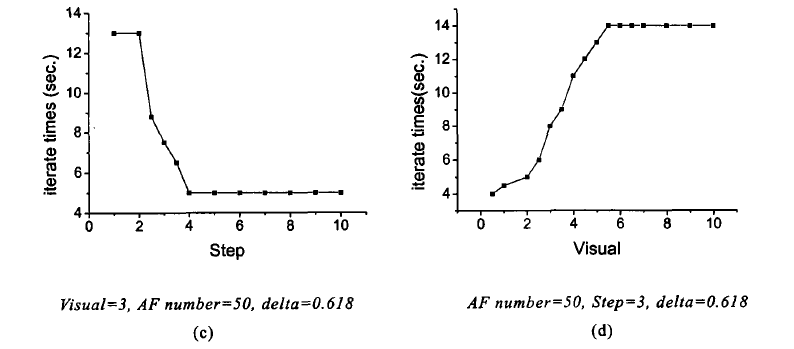
\includegraphics[height=0.5\textheight]{pic/fish7.png}
\end{figure}
\begin{figure}
\centering
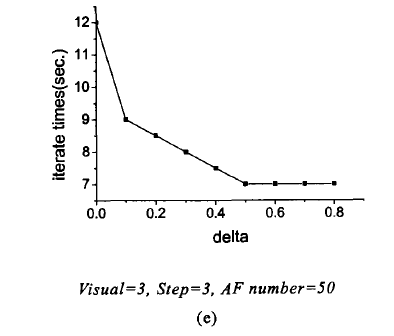
\includegraphics[height=0.5\textheight]{pic/fish8.png}
\end{figure}
\end{frame}

\begin{frame}
\frametitle{算法对照}
\small{遗传算法作为具有全局优化能力的代表算法之一,受到了长期的、广泛的关注,作者将鱼群算法与之进行了比较。由于这两种算法都存在一定的随机性,因此,在对照中分别进行了10组实验,最后将结果求平均,横坐标为各算法中迭代的次数。在本实验中,鱼群算法的参数同上;遗传算法中,编码长度为10,交叉位数为4,变异位数为2。图2.7展示了实验的结果;为了增强可比性,在对照1中,鱼群算法的人工鱼个体数为10,遗传算法的种群数为10;在对照2中,鱼群算法的人工鱼个体数为50,遗传算法的种群数为50。可见,鱼群算法中当人工鱼个体的数目较少时,还不能体现出它的优势,当然,对于遗传算法来说,种群数较少时也具有容易陷入局部极值和早熟的可能;当人工鱼个体的数目增加时,鱼群算法的收敛速度得以提高,而遗传算法则由于种群数的增多减缓了进化的速度,可见鱼群算法中蕴含着集群智能的优势。}

\begin{figure}
\centering
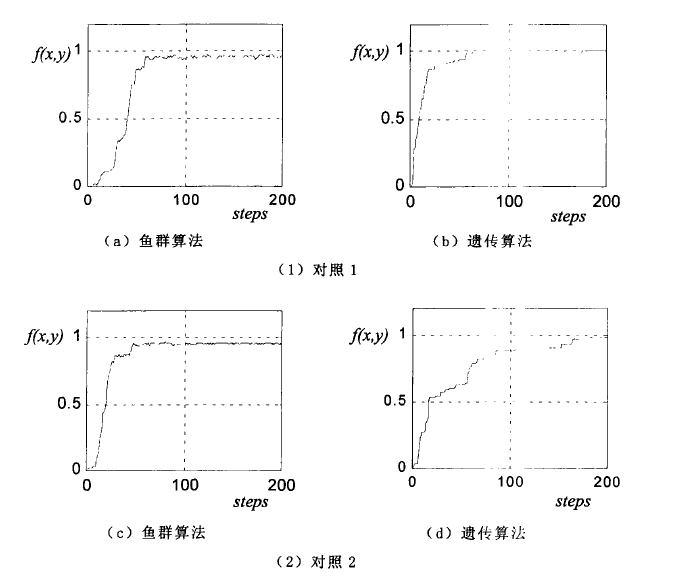
\includegraphics[width=0.7\textwidth]{pic/fish14.png}
\caption{鱼群算法与遗传算法的比较}
\end{figure}

\end{frame}

\begin{frame}
	\frametitle{算法特点}
	\begin{itemize}
		\item{算法只需要比较目标函数值,对目标函数的性质要求不高}
		\item{算法对初值的要求不高,初值随机产生或设定为固定值均可以}
		\item{算法对参数设定的要求不高,有较大的容许范围}
		\item{算法具备并行处理的能力,寻优速度较快}
		\item{算法具备全局寻优的能力}
	\end{itemize}
\end{frame}
\begin{frame}
	\frametitle{算法应用}	
	\begin{itemize}
		\item{组合优化问题}
		\item{分解协调问题}
	\end{itemize}
\end{frame}

\begin{frame}
\frametitle{组合优化问题——算法原理}
算法的原理与基本鱼群算法一致,在描述和实现中有些地方进行了适当的调整。如为了算法的简便易行,最优值的获取方式采用了跟踪记录最优个体状态的方法,因此,引入了公告板($AF\underline{\hspace{0.5em}}bulletin$)用来记录最优状加声,决妒第三章组合优化问题的人工鱼群算法应用43-态;为了解决带约束的优化问题,引入了约束行为($AF\underline{\hspace{0.5em}}subject$),扩展了算法的适用范围;为了更有效的增强算法的效能,用移动策略($AF\underline{\hspace{0.5em}}movestrategy$)替代了行为评价。\\
约束行为:在寻优过程中,由于聚群行为、随机行为等操作的作用,容易使得人工鱼的状态变得不可行,这时就需要加入相应的约束来对其进行规整化,使它们由无效状态或不可行状态转变成可行的。\\
\hspace{2em}公告板:公告板用来记录最优人工鱼个体的状态。各人工鱼个体在寻优过程中,每次行动完毕就检验自身状态与公告板的状态,如果自身状态优于公告板状态,就将公告板的状态改写为自身状态,这样就使公告板记录下历史最优的状态。\\
\hspace{2em}移动策略:移动策略是原行为评价的一种延伸,可以依旧采用原行为评价的模式,也可以采取一定的行动策略,如先进行追尾行为,如果没有进步再进行觅食行为,如果还没有进步则进行聚群行为,如果依然没有进步就进行随机移动行为。
\end{frame}

\begin{frame}
\frametitle{计算实例}
旅行商问题(TSP,travelingsalesman problem)是一个典型的组合优化问题,并且是NP一hard问题,下面就以对称距离的TSP问题为例来验证算法的性能。\\
旅行商问题就是一个商人欲到n个城市推销商品,每两个城市之间的距离为$d_{i,j}$,如何选择一条道路使得商人每个城市走一遍后回到起点所走过的路径最短。它的数学模型描述为:\\
$min\sum_{i\ne j}d_{ij}x_{ij}$\\
$s.t.\sum_{j=1}^n x_{ij}=1,i=1,2,…,n,$\\
\indent $\sum_{j=1}^n x_{ij}=1,j=1,2,…,n$\\
\indent $\sum_{i,j \in s} x_{ij}\le |s|-1,2\le|s|\le n-2, s\subset \{ 1,2,…,n\},$\\
\indent $x_{ij}\in \{0,1\},i,j=1,2,…,n,i\ne j$
\end{frame}

\begin{frame}
\frametitle{计算实例——TSP}
\small{数据来源:http://www.uni-heidelberg.de/iwr/comopt/software/TSPLIB95/;在对城市Ulysses22(22个城市)的寻优中,算法参数为$AF\underline{\hspace{0.5em}}Number=9, Visual=16,trynumber=500$,200步迭代的计算时间约为11秒;在对Att48(48个城市)的寻优中,$AF\underline{\hspace{0.5em}}Number=9, Visual=45, trynumber=300$,迭代计算时间大约为70秒。\\
在仿真实验中,为了反映算法对组合优化问题的解决能力,没有针对TSP问题的特点添加任何的启发规则,完全依靠人工鱼群算法对解空间的寻优能力,可见,人工鱼群算法具有较快的收敛速度,但是随着问题规模的扩大,其寻优的精度会有所降低,这是有待改进的地方。}
\begin{columns}
	\column{0.5\textwidth}
	\begin{figure}
	\centering
	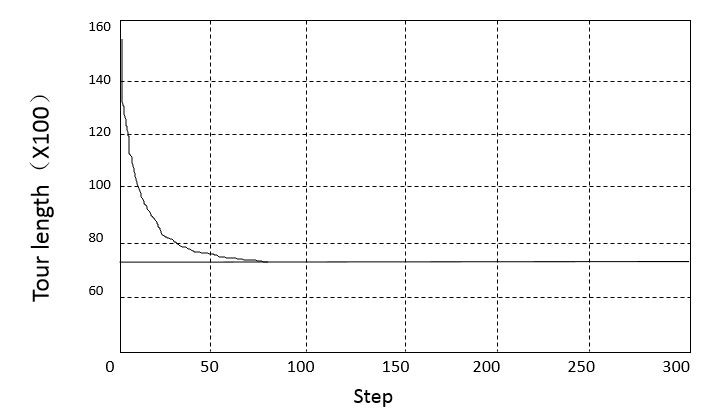
\includegraphics[width=1.0\textwidth]{pic/fish4.png}
	\caption{Ulysses 22 城市TSP问题的寻优曲线}
	\end{figure}
	\column{0.5\textwidth}
	\begin{figure}
	\centering
	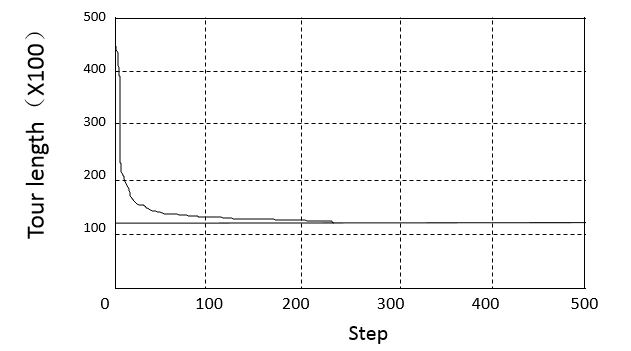
\includegraphics[width=1.0\textwidth]{pic/fish5.png}
	\caption{Att48 城市TSP问题的寻优曲线}
	\end{figure}

\end{columns}
通过对TSP的仿真可以看出,人工鱼群算法在离散问题的解决方面也具备较快的收敛能力。作为一种新型的智能优化方法,它还有许多需要进一步改进的地方;
其较快的收敛速度,可以应用于一些有实时性要求的地方;对于一些精度要求不高的场合,也可以用它快速的得到一个可行解;另外,对问题的了解不必很深,甚至不需要问题的精确描述,也使得它的应用范围得以延伸。
\end{frame}

\begin{frame}
\frametitle{基于分解协调的人工鱼群算法}
通常,大系统可以通过变换分解为一些子系统,一般子系统之间会存在一定的藕合关系,如果没有祸合关系,那么问题会变得更加简单了,对各子系统分别寻优的解将是大系统的最优解。在对大系统进行分解后,根据各子系统来设计各类人工鱼相应的寻优目标和行为,从而将鱼群分为多个不同的种类。设想用刃类鱼来分别表示这万个子系统,然后用万类鱼群通过基本鱼群算法分别求各子系统的最优解。通常情况下,由于子系统间和约束条件的祸合性,所得的解都不是所期望的全局最优解。而随着鱼群协调行为的引入,这个问题得到了很好的解决。\\
算法采用自下而上的设计方法,设计的关键就是底层的人工鱼个体行为的实现,算法的进行也就是人工鱼个体的自适应的行为活动,最优解将在该过程中突现出来。算法中每条人工鱼作为一个实体,该实体中封装着自身的状态和行为,实体每活动一次就是算法的一次迭代。
\end{frame}

\begin{frame}
\frametitle{计算实例}
如图所示的换热系统,四股热流的热容流量均为15000W/$^{\circ}$C,流线\uppercase\expandafter{\romannumeral3}的冷流体(进口温度150$^{\circ}$C)的热容流量为13500W/$^{\circ}$C,其余两股冷流体的热容流量为10000W/$^{\circ}$C。位于流线\uppercase\expandafter{\romannumeral3}上的换热器的传热系数均为135W/($m^2\cdot ^{\circ}C $),其余的换热器的传热系数均为100W/($m^2\cdot ^{\circ}C $).要求三股冷流体的出口温度分别达到400$^{\circ}$C,450$^{\circ}$C,500$^{\circ}$C。求换热面积最小时的换热面积最优分配。
\begin{figure}[H]
\centering
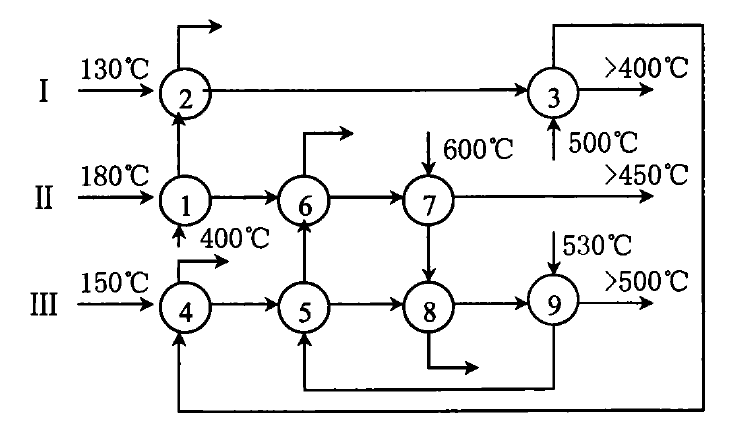
\includegraphics[width=0.5\textwidth]{pic/fish15.png}
\caption{换热器系统}
\end{figure}
\end{frame}

\begin{frame}
\frametitle{计算实例}
\small{计算结果:在实验中每类人工鱼的数目在10个左右时就能稳定的收敛到满意的解域,移动步长tSeP的取值从10一200,视野范围visual的取值从20一400都能保证比较稳定的收敛,并且迭代100次的时间约5秒钟。由于算法中存在一定的随机性,所以为了验证算法的收敛性能,连续进行了多次计算。参数取值为:每类人工鱼的个数均为15个,移动步长Step=50,视野范围Visual=300,在仿真中没有使用拥挤度因子$\delta$。如图所示分别是连续10次的计算结果进行平均后所得的迭代收敛曲线以及所得结果最优的一次计算过程的迭代收敛曲线。}
\begin{figure}[H]
\centering
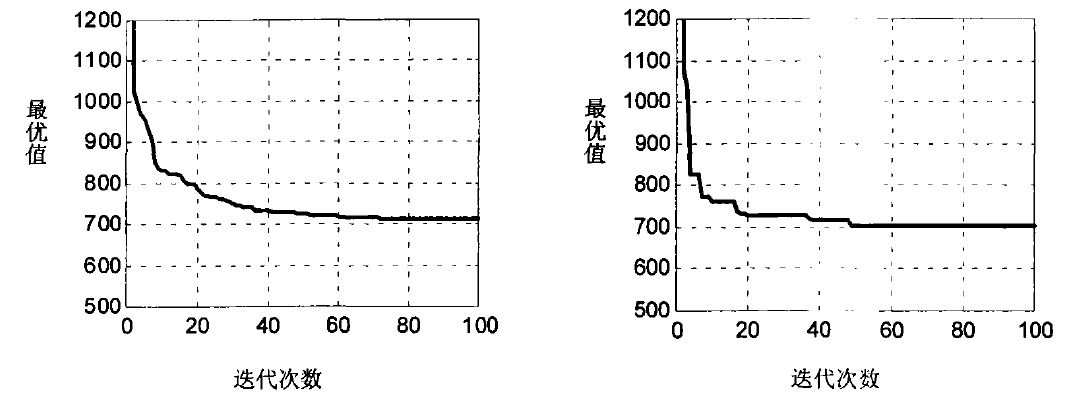
\includegraphics[width=0.8\textwidth]{pic/fish16.png}
\caption{计算结果收敛曲线,(左)平均,(右)最优}
\end{figure}
\end{frame}

\begin{frame}
\frametitle{计算实例}
从以上的计算实例可以看出,采用基于分解协调思想的人工鱼群算法具有以下几个特点:
\begin{itemize}
\item 算法对变量的初始值无要求,可以是随机产生的值,包括无效解也可以;
\item 算法中仅仅使用了目标函数的函数值,对函数的性质没有特殊要求;
\item 算法的收敛性好,大都能收敛到比较满意的解;
\item 参数的敏感性低,算法中参数的选择要求不高,参数的变动对结果的影响也不大;
\item 分解与协调思想的引入为复杂的大系统的优化问题的解决提供了一条可行的途径。
\end{itemize}
\end{frame}

\begin{frame}
\frametitle{分析思考}
在前面部分的论述中可以看出,鱼群算法在解决问题时存在一些优点:\\
\begin{itemize}
\item 算法中只需要比较目标函数值,因此对目标函数要求不高;
\item 算法对初值的要求不高,初值随机产生或设定为固定值均可以;
\end{itemize}
\indent 算法对参数设定的要求不高,有比较大的容许范围;同时,它也存在一些有待改进的地方:
\begin{itemize}
\item 随着人工鱼数目的增多,将会需求更多的存储空间,也会造成计算量的增长;
\item 由于视野和步长的随机性和随机行为的存在,使得寻优的精度难以很局;
\item 由于鱼群模式可以采用面向对象的方式来实现,所以,对功能的扩展和改造有着良好的基础。
\end{itemize}
\end{frame}

\begin{frame}
	\frametitle{参考文献}
	\begin{thebibliography}{123456} 
	\bibitem{fish_bib1} 李晓磊,邵之江,钱积新.一种基于动物自治体的寻优模式:鱼群算法[J].系统工程理论与实践,2002,22(11):32 -38.
	\bibitem{fish_bib2} 李晓磊.一种新到的智能优化方法———人工鱼群算法[D].杭州:浙江大学,2003.
	\bibitem{fish_bib3}李晓磊,钱积新.基于分解协调的人工鱼群优化算法研究[J].电路与系统学报,2003,8(1) : 1 -6.
	\end{thebibliography}
\end{frame}